\documentclass[10pt,a4paper]{article}

\usepackage[utf8]{inputenc}
\usepackage[T1]{fontenc}
\usepackage[english]{babel}
\usepackage{lmodern}
\usepackage{textcomp} % para símbolos como º
\usepackage{amsmath, amssymb}
\usepackage{graphicx}
\usepackage{booktabs}
\usepackage{siunitx}
\usepackage{hyperref}
\usepackage{xcolor}
\usepackage{listings}
\usepackage{enumitem}
\usepackage{float}
\usepackage{microtype}

\lstdefinestyle{CStyle}{
  language=C,
  basicstyle=\ttfamily\small,
  keywordstyle=\color{blue},
  commentstyle=\color{gray},
  numbers=left,
  numberstyle=\tiny,
  stepnumber=1,
  numbersep=5pt,
  frame=single,
  breaklines=true,
  showstringspaces=false
}

\title{\textbf{Project Assignment I: All-Pairs Shortest Path (APSP)}\\
\large Repeated Squaring and Fox’s Algorithm using MPI}

\author{Sérgio Cardoso up202107918 \\ Kathleen Soares up201903010}
\date{\today}

\begin{document}

\maketitle

\begin{abstract}
This report presents a parallel implementation of the \emph{All-Pairs Shortest Path} (APSP) problem using the min-plus product and the \emph{Repeated Squaring} method combined with Fox's algorithm on MPI. The program, developed in C, employs a distributed grid of \(Q \times Q\) processes (\(P = Q^2\)). The main design choices, communication strategy, and preliminary performance results are presented.
\end{abstract}

\section{Introduction}
This project computes the shortest distances between all pairs of vertices in a weighted directed graph, represented by an adjacency matrix \(A\). The graph is represented by an adjacency matrix \(A\), where each entry \(A_{ij}\) corresponds to the edge weight or infinity when no connection exists.
 The algorithm applies the min-plus product and the \emph{Repeated Squaring} method, with each multiplication parallelized using Fox’s algorithm on MPI.

\section{Algorithmic Base}

\subsection{Min-Plus Product}
The min-plus product of matrices \(A\) and \(B\) is defined as:
\[
C_{ij} = \min_k (A_{ik} + B_{kj})
\]
This replaces the standard addition by the minimum and multiplication by addition, propagating minimal path distances. In the code, this logic appears in \texttt{local\_minplus\_mm()}, where each process computes its local block of \(C\) from the corresponding blocks of \(A\) and \(B\).

\subsection{Repeated Squaring}
The method applies the min-plus product repeatedly (\(A^2, A^4, A^8, \ldots\)) until \(2^k \ge N-1\). Each iteration calls \texttt{fox\_minplus()}, ensuring all shortest paths are obtained.

\subsection{Fox's Algorithm}
Fox's algorithm is used to multiply blocks of matrices in parallel. The matrix is divided into sub-blocks \((N/Q) \times (N/Q)\), distributed among the processes arranged in a Cartesian grid. Each process performs, in each phase, a broadcast of blocks of \(A\) along the row and a circular rotation of blocks of \(B\) along the column, computing the local part of \(C\) with the min-plus operation.

\begin{figure}[H]
  \centering
  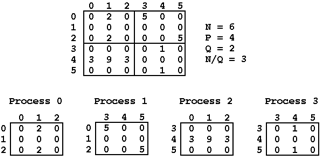
\includegraphics[width=0.8\textwidth]{matrix_foxImage.png}
  \caption{Example of process grid and communication pattern in Fox's algorithm.}
  \label{fig:fox_algorithm}
\end{figure}

\section{Implementation Details}

\subsection{Main Steps}
\begin{enumerate}
  \item \textbf{Input:}  
  Process 0 reads the adjacency matrix. Zeros outside the diagonal are replaced by \texttt{INF = 1e9} to represent no connection.
  
  \item \textbf{Grid setup:}  
  A 2D Cartesian topology is created. The program checks that \(p = q^2\); otherwise, it prints an error and terminates.
  \item \textbf{Padding:}  
  If \(N\) is not a multiple of \(q\), the matrix is automatically padded to \(N_{pad}\) to match the grid size.
  
  \item \textbf{Distribution:}  
  The (padded) matrix is divided into blocks and assigned to processes according to grid coordinates \((i, j)\).
  \item \textbf{Parallel multiplication:}  
  In each step:
  \begin{itemize}[noitemsep]
    \item block \(A\) is broadcast along the row;
    \item each process computes its local min-plus product with block \(B\);
    \item block \(B\) is rotated vertically using \texttt{MPI\_Sendrecv\_replace}.
  \end{itemize}
\item \textbf{Repeated squaring:}  
  The algorithm repeats min-plus multiplications until \(2^k \ge N-1\).

\item \textbf{Result:}  
  Process (0,0) gathers the final matrix and prints it, replacing infinite values by zeros.
\end{enumerate}

 \subsection*{Input Validation and Padding}
The program validates the number of processes (\(p=q^2\)) and ensures \(N\) is positive and even.  
When \(N\) is not divisible by \(q\), the matrix is padded to size \(N_{pad} = \lceil N/q \rceil \times q\) with INF values and zeros on the diagonal, ensuring compatibility with any process grid.

\section{Main Implemented Functions}

\subsection{\texttt{grid\_setup}}
Creates an Cartesian topology of processes and the row and column sub-communicators using \texttt{MPI\_Cart\_create} and \texttt{MPI\_Cart\_sub}, 
assigning to each process coordinates \((my\_row, my\_col)\).

\subsection{\texttt{local\_minplus\_mm}}
Executes the min-plus product between two local blocks \(A\) and \(B\), accumulating the result in \(C\):
\[
C[i][j] = \min_k(A[i][k] + B[k][j])
\]
Unnecessary additions involving infinite values are avoided to reduce computational cost.

\subsection{\texttt{fox\_minplus}}
Implements the core of Fox's algorithm.  
At each iteration:
\begin{itemize}
  \item the root process of the row broadcasts its block \(A\);
  \item each process calculates its local contribution via \texttt{local\_minplus\_mm};
  \item the blocks \(B\) are rotated vertically with \texttt{MPI\_Sendrecv\_replace}.
\end{itemize}

\subsection{\texttt{copy\_block\_out} and \texttt{copy\_block\_in}}
Auxiliary functions that copy blocks between the global (padded) matrix and the local submatrices, preserving the original data layout.

\subsection*{Communication Strategy}
Each process broadcasts blocks with \texttt{MPI\_Bcast} along rows and rotates them with \texttt{MPI\_Sendrecv\_replace} along columns.  
Row and column subcommunicators (\texttt{MPI\_Cart\_sub}) ensure synchronization and avoid deadlocks.

\section{Error Handling and Robustness}
The code handles invalid input situations such as:
\begin{itemize}
  \item negative values or \(N = 0\);
  \item non-perfect square number of processes;
 \item incompatible padding configuration.
\end{itemize}
Each memory allocation is checked and aborts execution with an error message in case of failure.

\section{Performance Evaluation}
Execution time and speedup were measured for 1, 4, 9, 16, and 25 processes.  
Only computation and communication times were considered (I/O excluded).  

\begin{table}[H]
  \centering
  \caption{Execution time (ms) and speedup for different process counts.}
  \begin{tabular}{ccc}
    \toprule
    \textbf{Processes} & \textbf{Time (ms)} & \textbf{Speedup} \\
    \midrule
    1  & x & 1.00 \\
    4  & x & x \\
    9  & x & x \\
    16 & x & x \\ 
    25 & x & x \\
    \bottomrule
  \end{tabular}
\end{table}

Speedup remains close to linear up to 16 processes, with communication overhead becoming dominant for larger configurations.

\section{Main Difficulties and Comments}
The main challenges faced during development were:
\begin{itemize}
  \item ensuring compatibility between matrix size and the number of MPI processes (\(N \bmod Q = 0\));
  \item debugging Fox's communication pattern, particularly the vertical rotation using \texttt{MPI\_Sendrecv\_replace};
  \item implementing and testing automatic padding while keeping the code efficient and readable;
  \item validating numerical accuracy for small test cases and avoiding overflow for large distance values.
\end{itemize}

Overall, the project was valuable to strengthen understanding of distributed programming with MPI, providing practical experience in process synchronization, load balancing, and scalability analysis.
 
As a suggestion, a visual tool to display matrix partitioning and message flow could help future students better understand process decomposition.

\section{Conclusions}
The parallel APSP implementation using Fox’s algorithm with min-plus multiplication proved efficient and scalable.  
Automatic padding and validation improve robustness and flexibility.  
This project consolidated concepts of distributed computation, communication patterns, and performance analysis in MPI.

\begin{thebibliography}{9}
\bibitem{cormen2009introduction}
Cormen, T. H., Leiserson, C. E., Rivest, R. L., \& Stein, C. (2009).
\textit{Introduction to Algorithms} (3rd ed.).
MIT Press.

\bibitem{fox1987}
Fox, G. C., Otto, S. W., \& Hey, A. J. (1987).
\textit{Matrix algorithms on a hypercube I: Matrix multiplication}.
Parallel Computing, 4(1), 17–31.

\bibitem{pacheco1998}
Pacheco, P. S. (1998).
\textit{A User's Guide to MPI}.
San Francisco: Department of Mathematics, University of San Francisco.
  \end{thebibliography}

\vspace{0.3cm}
  
\textit{Note: The complete source code (\texttt{fox.c}) is attached in the ZIP file submitted along with this report.}

\end{document}